\documentclass[10pt,twocolumn]{article}

\usepackage{graphicx}
\usepackage{amsmath}
\usepackage{amssymb}
\usepackage{hyperref}
\usepackage{geometry}
\usepackage{enumitem}
\usepackage{booktabs}
\usepackage{multirow}

\geometry{letterpaper, margin=0.75in}

\title{\textbf{Midterm Report: Image Captioning and Weather Analysis}}
\author{Siyuan Jing \quad Haonan Wu \quad Rui He\\
Boston University\\
\texttt{siyuan16@bu.edu \quad whn17@bu.edu \quad rhe1012@bu.edu}}
\date{}

\begin{document}

\maketitle

\section{Task Overview}
Our system generates image captions and predicts weather cues \emph{simultaneously}. A shared CLIP backbone feeds two parallel heads: (1) a CLIP-prefix-to-GPT decoder for natural-language captions, and (2) a weather classifier that enriches the caption with environmental context. Aligning both outputs mitigates the mode-collapse failure we observed when captioning operated alone and ensures user-facing responses reflect scene conditions.

\medskip
\noindent The end-to-end training pipeline couples the caption and weather branches:
\begin{enumerate}[leftmargin=1.5em]
    \item \textbf{COCO dataset} $\rightarrow$ \texttt{01\_Database\_to\_Clip.py}
    \item $\rightarrow$ \texttt{CLIP\_Pro\_train\_merged.pkl} / \texttt{CLIP\_Pro\_val\_merged.pkl}
    \item $\rightarrow$ \texttt{02\_Train\_Plus.py}
    \item $\rightarrow$ \texttt{clip\_pro\_prefix-best.pt} (model weights)
    \item $\rightarrow$ \texttt{03\_Predict.py} (caption generation)
    \item $\rightarrow$ \texttt{04\_Evaluation.py} / \texttt{05\_Score.py} (metrics)
\end{enumerate}

Joint inference produces captions conditioned on real-time weather predictions; users receive answers that combine textual descriptions with climate indicators (e.g., ``A person walking with an umbrella. Weather: rainy (95\%).'').

The weather branch currently attains $\sim$40\% accuracy. Indoor-heavy validation data and ambiguous sky cues limit performance, motivating targeted data augmentation to balance both tasks.

\begin{figure}[t]
    \centering
    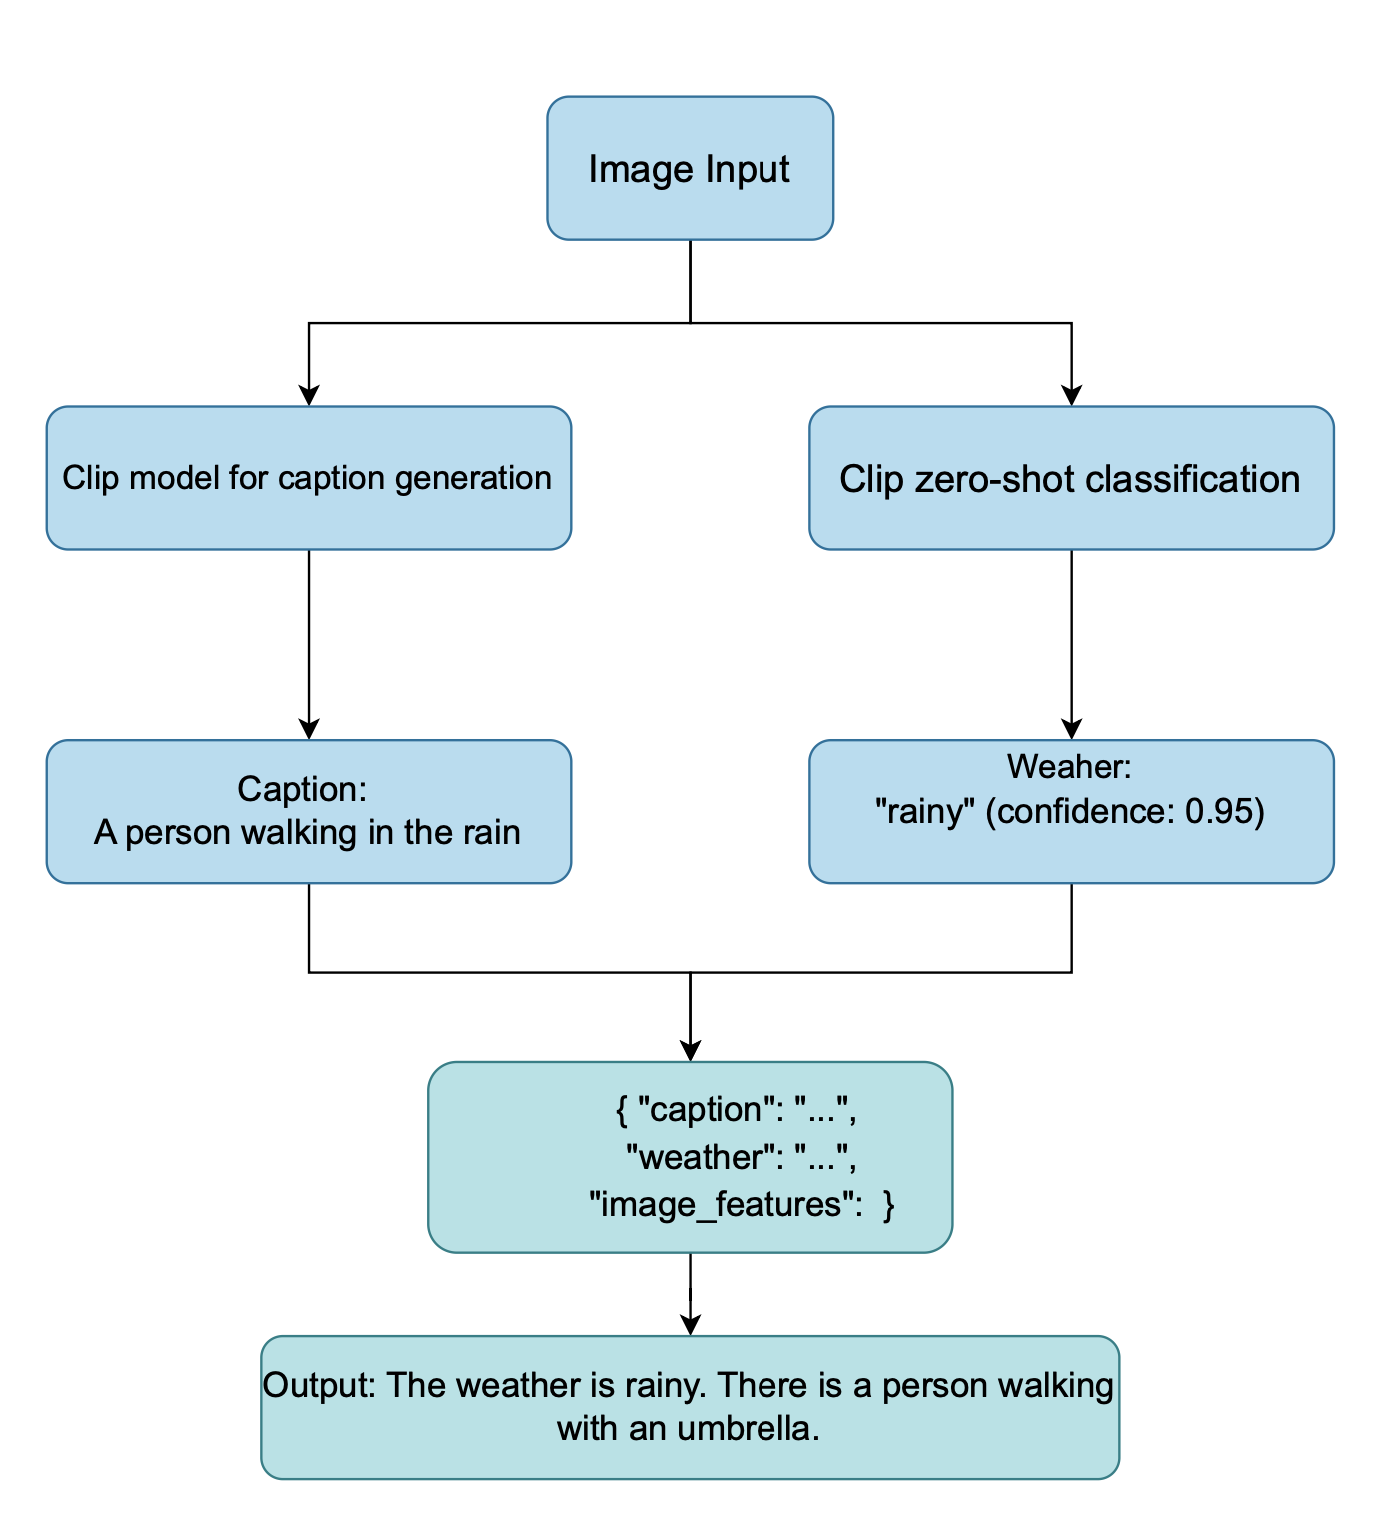
\includegraphics[width=\linewidth]{flownap.png}
    \caption{System overview highlighting dual-branch captioning and weather analysis.}
    \label{fig:flow}
\end{figure}

\section{Background and Related Work}
\subsection{Contrastive Language-Image Pretraining (CLIP)}
CLIP~\cite{mokady2021clipcap} is a vision-language model trained using contrastive loss on 400M image-text pairs collected from the web. It contains a dual-encoder architecture with a visual encoder (ResNet/ViT) and a text transformer. Mokady et al.~\cite{mokady2021clipcap} demonstrate that CLIP embeddings can be projected into the input space of GPT-2, providing a prefix that conditions subsequent caption generation. This motivates our adoption of CLIP as the visual backbone.

\subsection{Generative Pre-trained Transformer 2 (GPT-2)}
GPT-2~\cite{radford2019language} is a transformer-decoder-only architecture optimised for autoregressive language modeling. Its self-attention mechanism captures long-range dependencies more efficiently than recurrent networks. We therefore select GPT-2 as the linguistic decoder in our pipeline, expecting coherent, contextually grounded captions.

\subsection{Multi-Head Attention Mechanism}
Following Vaswani et al.~\cite{vaswani2017attention}, multi-head attention enables the model to attend to multiple representation subspaces. We employ cross-modal attention between CLIP embeddings and the GPT-2 decoder, allowing the system to focus on salient visual cues when generating each token. This design has proven advantageous in prior captioning frameworks and we observe similar benefits.

\section{Experimental Progress}
\subsection{Caption Generation}
We fine-tune the CLIP-prefix-to-GPT-2 mapping using COCO training splits. Preliminary outputs demonstrate syntactically fluent captions, yet content diversity remains limited due to mode collapse. We are exploring:
\begin{itemize}[leftmargin=1.5em]
    \item Noise injection and augmentation (cf.~\cite{nukrai2022text}) to encourage broader caption distributions.
    \item Temperature and nucleus sampling adjustments during decoding.
    \item Curriculum learning on curated subsets with higher caption entropy.
\end{itemize}

\subsection{Weather Classification}
The weather branch uses CLIP-derived features with a lightweight classifier to predict labels such as \emph{sunny}, \emph{rainy}, or \emph{snowy}. Accuracy plateaued around 40\%, likely due to weak weather signals in indoor imagery. Planned improvements include:
\begin{enumerate}[leftmargin=1.5em]
    \item Augmenting training data with weather-focused datasets.
    \item Incorporating temporal cues where available.
    \item Applying label smoothing and class re-balancing.
\end{enumerate}

\section{CLIP Zero-Shot Weather Classification}
Recent advances in zero-shot CLIP classification~\cite{sammani2024interpreting,qian2024online} inspire a complementary evaluation pathway. We implement a CLIP-driven classifier that operates without additional weather labels, generating predictions from textual prompts that describe weather conditions.

\subsection{Inference Pipeline}
\begin{enumerate}[leftmargin=1.5em]
    \item \textbf{Image encoding}: Extract visual embeddings using the CLIP vision encoder.
    \item \textbf{Text encoding}: Convert weather descriptions into embeddings with the CLIP text encoder.
    \item \textbf{Similarity scoring}: Compute cosine similarities between image and text embeddings.
    \item \textbf{Probability normalization}: Apply softmax to transform similarities into a probability distribution.
    \item \textbf{Result output}: Return the top-1 weather label alongside class probabilities.
\end{enumerate}

\subsection{Prompt Engineering}
We enrich the prompt set with descriptive suffixes to emphasise weather cues, following recommendations from prior zero-shot studies. Table~\ref{tab:weather-prompts} lists the prompts currently deployed.

\begin{table}[h]
    \centering
    \caption{Weather categories and associated prompt augmentations used for CLIP zero-shot inference.}
    \label{tab:weather-prompts}
    \begin{tabular}{ll}
        \toprule
        Weather type & Prompt suffix \\
        \midrule
        Sunny   & \textit{``on a sunny day''} \\
        Rainy   & \textit{``in the rain''} \\
        Snowy   & \textit{``in the snow''} \\
        Cloudy  & \textit{``under cloudy skies''} \\
        Foggy   & \textit{``in foggy conditions''} \\
        Stormy  & \textit{``during a storm''} \\
        Overcast& \textit{``under overcast skies''} \\
        Clear   & \textit{``on a clear day''} \\
        \bottomrule
    \end{tabular}
\end{table}

\subsection{Output Format}
Inference produces: (i) the most probable weather type (e.g., ``Rainy''), (ii) confidence scores (e.g., 95\%), and (iii) the full probability distribution visualised as a bar chart for interface consumption. These outputs can dynamically adjust caption phrasing to align with environmental context.

\section{Next Steps}
\begin{itemize}[leftmargin=1.5em]
    \item Address mode collapse by experimenting with contrastive regularizers and diverse beam search variants.
    \item Enhance weather detection through specialized datasets and multimodal feature fusion (e.g., integrating horizon detectors or sky segmentation).
\end{itemize}

\begin{thebibliography}{99}
\bibitem{nukrai2022text}
D.~Nukrai, R.~Mokady, and A.~Globerson, ``Text-Only Training for Image Captioning using Noise-Injected CLIP,'' 2022. \url{https://doi.org/10.48448/n7sq-p557}.

\bibitem{mokady2021clipcap}
R.~Mokady, A.~Hertz, and A.~H. Bermano, ``ClipCap: CLIP Prefix for Image Captioning,'' 2021. \url{http://arxiv.org/abs/2111.09734}.

\bibitem{radford2019language}
A.~Radford, J.~Wu, R.~Child, D.~Luan, D.~Amodei, and I.~Sutskever, ``Language Models are Unsupervised Multitask Learners,'' OpenAI Technical Report, 2019.

\bibitem{vaswani2017attention}
A.~Vaswani, N.~Shazeer, N.~Parmar, J.~Uszkoreit, L.~Jones, A.~N. Gomez, {\L}.~Kaiser, and I.~Polosukhin, ``Attention Is All You Need,'' in \emph{Advances in Neural Information Processing Systems}, 2017.

\bibitem{chen2015cococaptions}
X.~Chen, H.~Fang, T.-Y. Lin, R.~Vedantam, S.~Gupta, P.~Doll{\'a}r, and C.~L. Zitnick, ``Microsoft COCO Captions: Data Collection and Evaluation Server,'' arXiv preprint arXiv:1504.00325, 2015.

\bibitem{papineni2002bleu}
K.~Papineni, S.~Roukos, T.~Ward, and W.~J. Zhu, ``BLEU: A Method for Automatic Evaluation of Machine Translation,'' in \emph{Proceedings of ACL}, 2002.

\bibitem{vedantam2015cider}
R.~Vedantam, C.~L. Zitnick, and D.~Parikh, ``CIDEr: Consensus-based Image Description Evaluation,'' in \emph{Proceedings of CVPR}, 2015.

\bibitem{sammani2024interpreting}
F.~Sammani and N.~Deligiannis, ``Interpreting and Analysing CLIP's Zero-Shot Image Classification via Mutual Knowledge,'' in \emph{Proceedings of NeurIPS}, 2024. \url{https://doi.org/10.48550/arXiv.2410.13016}.

\bibitem{qian2024online}
Q.~Qian and J.~Hu, ``Online Zero-Shot Classification with CLIP,'' in \emph{Proceedings of ECCV}, 2024. \url{https://doi.org/10.48550/arXiv.2408.13320}.
\end{thebibliography}

\end{document}

